\section*{Aufgabe 1.2}
\subsection*{Angabe}
	Von einem Signal $x\leftn[n\right]$ sei der gerade Anteil $x_g\leftn[n\right]$ und das Signal $x_1\leftn[n\right]$ gegeben. Bestimmen Sie den ungeraden Anteil des Signals $x\leftn[n\right]$.
	\begin{center}
		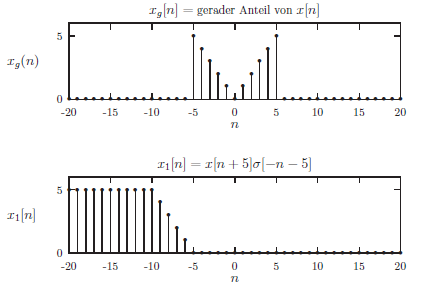
\includegraphics{1_2}
	\end{center}
\subsection*{Lösung}
	In diesem Beispiel wird der Einheitssprung $\sigma$ verwendet. Dieser ist definiert mit
	\[
		\sigma\leftn[n\right]=\left\{\begin{array}{cl} 0, & n<0\\1, & n\ge 0 \end{array} \right.
	\]
	Betrachten wir nun die Funktion $x_1\leftn[n+5\right]\sigma \leftn[-n-5\right]$, lässt sich leicht erkennen, dass der Einheitssprung $\sigma \leftn[-n-5\right]$ nur bei $n\le -5$ Werte zulässt. Wir können das Signal $x\leftn[n\right]$ vorerst nur bis zu dieser Stelle rekonstruieren.\\
	Der Ausdruck $x\leftn[n+5\right]$ verschiebt das Signal $x\leftn[n\right]$ nach links. Es lässt sich aus dem Plot herauslesen, dass $x\leftn[n\right]$ bis zu $n=-5$ den Wert $5$ erzeugt, und anschließend linear von -5 gegen 0 abfällt. Wir können definieren:
	\[
		x\leftn[n\right]=\left\{\begin{array}{cl} 5, & n < -5\\-n, & -5\le n<0\\?, & n\ge 0 \end{array} \right.
	\]
	Nun fehlt uns noch Definition für positive n-Werte. Dabei bedienen wir uns dem angegebenen $x_g\leftn[n\right]$ und der Umformung:
	\[
		x_g\leftn[n\right]=\frac{1}{2} \left(x\leftn[n\right]+x\leftn[-n\right]\right)\Leftrightarrow x\leftn[n\right]=2x_g\leftn[n\right]-x\leftn[-n\right]
	\]
	Das heißt, dass wir alle positiven Signalwerte von $x\leftn[n\right]$ berechnen können, indem wir die geraden Anteile $x_g\leftn[n\right]$ und die negativen Signalwerte $x\leftn[-n\right]$ kennen. Nun muss nur noch der Parameter $n$ für $n \ge 0$ variiert werden.
	\begin{center}
		\begin{tabular}{|c|c|c|c|c|c|c|c|c|c|c|c|}
		\hline n & 0 & 1 & 2 & 3 & 4 & 5 & 6 & 7 & 8 & 9 & 10 \\
		\hline $2x_g\leftn[n\right]$ & 0 & 2 & 4 & 6 & 8 & 10 & 0 & 0 & 0 & 0 & 0 \\
		\hline $x\leftn[-n\right]$ & 0 & 1 & 2 & 3 & 4 & 5 & 5 & 5 & 5 & 5 & 5 \\
		\hline $x\leftn[n\right]$ & 0 & 1 & 2 & 3 & 4 & 5 & -5 & -5 & -5 & -5 & -5 \\ 
		\hline 
		\end{tabular} 
	\end{center}
	Somit können wir $x\leftn[n\right]$ vollständig definieren:
	\[
		x\leftn[n\right]=\left\{\begin{array}{cl} 5, & n < -5\\|n|, & -5 \le n\le 5\\-5, & n>5 \end{array} \right.
	\]
	\begin{figure}[!h]	%1.2) x[n]
	\centering
		\begin{tikzpicture}[scale=0.5]
			\begin{axis}[
				xmin=-12, xmax=12,
				domain=-10:10,
				axis x line=middle,
				axis y line=middle,
				ylabel = {$x\leftn[n\right]$},
				y label style={at={(0.3,1)}},
				xlabel = $n$,
	       		xtick={-10,-5,...,10},
				]
				\addplot+[ycomb,blue,thick,domain=-10:-6,samples=5,mark=o] {5};
				\addplot+[ycomb,blue,thick,domain=-5:0,samples=6,mark=o] {-x};
				\addplot+[ycomb,blue,thick,domain=1:5,samples=5,mark=o] {x};
				\addplot+[ycomb,blue,thick,domain=6:10,samples=5,mark=o] {-5};
			\end{axis}
		\end{tikzpicture}
	\end{figure}
	Im letzten Schritt berechnen wir uns nun die ungeraden Teilsignale $x_u\leftn[n\right]$.
	\[
		x_u\leftn[n\right]=\frac{1}{2} \left(x\leftn[n\right]-x\leftn[-n\right]\right)
	\]
	Daraus erhalten wir:
	\[
		x_u\leftn[n\right]=\left\{\begin{array}{cl} 5, & -5 < n\\0, & -5\le n \le 5\\-5, & 5<n \end{array} \right.
	\]
	\begin{figure}[!h]	%1.2) x_u[n]
	\centering
		\begin{tikzpicture}[scale=1]
			\begin{axis}[
				xmin=-12, xmax=12,
				domain=-10:10,
				axis x line=middle,
				axis y line=middle,
				ylabel = {$x_u\leftn[n\right]$},
				y label style={at={(0.3,1)}},
				xlabel = $n$,
	       		xtick={-10,-5,...,10},
				]
				\addplot+[ycomb,blue,thick,domain=-10:-6,samples=5,mark=o] {5};
				\addplot+[ycomb,blue,thick,domain=-5:5,samples=11,mark=o] {0};
				\addplot+[ycomb,blue,thick,domain=6:10,samples=5,mark=o] {-5};
			\end{axis}
		\end{tikzpicture}
	\end{figure}